\chapter{Implementation of k-Means in HyPer}\label{chapter:implementation}

\section{LLVM Code Compilation Fundamentals}

Before we look at the implementation of k-Means as an HyPer operator we first talk about the implementation of operators in HyPer in general. With this understanding we can then show how k-Means can be adjusted to be used in this programming model. One of the main observations when working with main memory databases is that, since all the data resides in main memory, query performance is much more dependent on the CPU costs of the query processing than on I/O time as in traditional systems. Therefore, query processing for HyPer has to be reinvented to achieve optimal performance in main memory systems.
Before a query is executed, most database systems translate a query into an algebraic expression and start evaluating and executing this algebraic plan. Traditionally, this plan is executed using the iterator model: Each physical operator produces a tuple stream and iterates to the next tuple by calling the next function of the operator. This iterator model works well for I/O dominated, traditional databases, where CPU consumption was not a limiting factor. However, for main memory databases, this is not perfect: First, next is called up to a million times, since it is called for every single tuple for each intermediate and final result. Since the call to next is usually a virtual call or a call via a function pointer, this call is more expensive than a regular call and reduces branch prediction of modern CPUs. And finally, the iterator model results often in a poor code locality and complex bookkeeping. This can be seen by the functionality of a table scan: As one tuple is produced one at a time, the table scan has to remember where in the compressed stream the current tuple is and jump to the corresponding decompression code when asked for the next tuple. 
In order to resolve this issues, Neumann proposes a new query compilation strategy for main memory databases, as used in HyPer. Instead of the operator centric approach of the iterator model, processing is now data centric. Therefore data can be kept in the CPU registers as long as possible, while the boundaries between the operators are more and more blurred. That means that each code fragment performs all actions on the given data, until the result has to be materialized, e.g. data is taken out of the registers. A code structure like this generates almost optimal assembly code, since all the relevant instructions for the given data are generated, and therefore, the data can be kept in the CPU registers.
HyPer uses a simple programming model for its operators in order to make  compilation as efficient as possible, while writing code remains understandable and maintainable for the developer: Each operator implements two functions, a consume and a produce function. The produce function asks the operator to produce its result tuples, which are then pushed to the next operator by calling its consume function. The next operator works the same way, after getting data by a consume call of the predecessor, it produces result tuples by calling its own produce function. Therefore, each operator gets its consume function called by its predecessor, calls its own produce function to compute the results and calls then the consume function of its successor, as shown in the sequence diagram in~\autoref{fig:consume_produce_sd}.


\begin{figure}[htsb]
  \centering
  \includegraphics[scale=0.6]{figures/consume_produce}
  \caption[Consume-Produce Sequence Diagram]{Consume-Produce Sequence Diagram.}\label{fig:consume_produce_sd}
\end{figure}


Therefore, this programming model pushes data towards the next operator, instead of pulling the data. This results in a much better code and data locality. Tuples are pushed from one operator to the next, therefore operators benefit from keeping the data in the CPU registers, which allows very cheap and efficient computation. Thus, most computation is done using the CPU registers, only when materializing data memory has to be accessed. Additionally, small code fragments are used to handle large amounts of data in tight loops leading to good code locality and therefore high performance.
Therefore, computation is very fast. However, what happens when data has to be materialized? Whenever we talk about taking tuples out of the CPU registers, i.e. materializing tuples in main memory, the operator pipeline breaks, therefore we call it a pipeline breaker: A pipeline breaker is any operator that takes an incoming tuple out of the CPU registers for further programming. Materializes an operator all incoming tuples before continuing processing, we call it a full pipeline breaker. An example is a join operator: One side of the join relations has to be materialized in main memory,  while the other relation can be scanned and probe the materialized data for join partners. Therefore, the join operator takes data out of the registers and is a pipeline breaker.
It is important to note that the consume produce functions are just an abstraction layer for the programmer and are used by the code generation to compile assembly code. In the assembly code there is not consume produce anywhere. Queries are compiled by parsing the query, translated it into algebra and optimized. In contrast to a traditional system, the algebra is now not translated into physical algebra and executed, but compiled by the code generation into an imperative program. For this programming step the consume produce model is used.
For compiling the algebraic expressions into machine code, the first approach was to generate C++ code and load the result as a shared library at runtime. This seems logical because HyPer is already written in C++: The shared library could access the data structures of the database system. On the other hand, compiling optimized C++ code is very slow, only compilation could already take several seconds for a complex query, which is too slow for a database system. Additionally, the C++ compiler does not offer total control over the generated code, e.g. overflow flags are not available. Therefore, queries are compiled into native machine code using the LLVM compiler framework. 
The Low Level Virtual Machine (LLVM) compiler framework generates portable assembler code, which can be executed directly using an optimizing  JIT compiler. With LLVM HyPer uses a very robust assembly code generation, e.g. pitfalls like register allocation are hidden by LLVM. Therefore the assembly code generation is very convenient compared to other compiler frameworks. Furthermore, only the LLVM JIT compiler translates the portable code into machine dependent code, leading to portable code across computer architectures. Since the LLVM assembler is strongly typed, many bugs can be caught in contrast to the original textual C++ code generation. Furthermore, LLVM produces highly optimized, extremly fast machine code and outperforms in some cases even hand-written code as the assembly language allows code optimization, hardware improvements and other tricks, that are hard to do in a high-level language as C++. All this requires usually only a few milliseconds as compilation time, compared to the seconds needed when using C++ compilers. 
Additionally, LLVM code is perfectly able to interact with C++, the main language of the HyPer database which is a big advantage. Even though LLVM code is robust and convenient to write compared to common assembler code, it is still more painful than writing code in a high-level language like C++. This enables us to implement the operators using both C++ and LLVM code, and reuse database logic like index structures, that are already implemented in C++. 
Therefore, everything complex like data structures, or complex algorithms are written in C++ and connected together by LLVM Code, where the C++ code is pre-compiled, while the LLVM Code is compiled at runtime dynamically. Apart from using C++ for parts of the operators, it also results in low query compilation times. An example is the Sort operator: The compare function, comparing two tuples by the rules of the sort query is dynamically generated in LLVM code, depending on the schema of the database and the values. As actual sort function, the built-in C++ sort is used. This is a great example of the mixed execution model using both C++ and LLVM Code.
Even though C++ and LLVM can be used implementing an operator, the operator is driven by LLVM code and uses C++ as convenience. For performance gains, it is important that the code that is executed for most of the tuples is pure LLVM code, even though calling C++ from time to time is acceptable. As already mentioned, staying in LLVM allows to keep the data in the CPU registers and is therefore the preferable way of executing a query. Calling an external function spills all registers to memory, which can be a bottleneck when doing this a million times, which is quite likely when using big amounts of data.
As conclusion, we now learned that the HyPer programming model for operators implements a consume produce model to push data towards the next operator. Furthermore, the LLVM compiler framework is used for code generation and can be combined with C++ code at runtime. 
One of the main challenges for the implementation of Data Mining algorithms, that are mostly complex, is how to divide the algorithm in LLVM and C++ code to gain optimal performance.
Parallel?


After acquiring a basic understanding of HyPer’s operator model, in particular the interaction of dynamically generated LLVM code and pre-compiled C++ code, we can talk about the actual implementation of k-Means. The most interesting part of implementing a complex operator like k-Means is the decision about how to implement the algorithm, either in LLVM or C++. 
This question is not trivial, because there are no strict rules and several possibilities. First, we look at tuples, e.g. when comparing tuples with each other in the sort operator, or the computation of a distance in the k-Means operator. Since the code has to handle different data types depending on the table schema, a dynamic generation of the code works best. For the other parts, like the implementation of a sort function or the combination of loops in k-Means, it is not so obvious where to put the code. In this work we present two different ways of implementing a k-Means Operator in HyPer, first an operator implementing the algorithm in C++ and uses only a few generated LLVM functions, e.g. to compute the distance. Secondly, a system is presented implementing k-Means almost entirely in LLVM. Only small parts, like picking random centers are implemented in C++. In the evaluation section we compare both implementation regarding the compile and execution time.


\section{Requirements and Constraints}

\section{Functionality}
Before we look about the technical implementation details in greater details, we discuss the functionality our k-Means operator, in particular the input and output parameters for calling k-Means. 
As input parameters, the user can specify the number of maximum iterations of the algorithm. If this parameter is omitted, the algorithm runs until convergence. For big data sets this is often a performance problem when only a few data points are changed from one iteration to the other, but all the distances from each data point to each center have to be computed for each additional iteration. Often the result is already accurate enough for a predefined number of iteration. Apart from an advantage regarding the running time, it is also important to specify the number of iterations for proper testing. In the following experiment section, we experiment the running time for ten iterations.
Further parameters are the initialization strategy and a verbose option. As initialization strategy, the user can select between random initialization and the k-Means++ initialization. The verbose option let the algorithm to compute and to print additional information about the k-Means algorithm.
As default output, an additional column is added to each data row presenting the cluster identifier of the data tuple as an integer. If the verbose option is active, statistics about the run are printed to the console. This information contain the number of iterations, the final center coordinates and the number of assigned data points and the sum of squared errors. 
The number of iterations is  important for comparing the running time of different k-Means algorithms in a fair manner. It is possible that one run converges after three iterations, while another one converges after seven iterations. The number of iterations is non-deterministic since we are using a random initialization strategy. For fair evaluation, the time per iterations is therefore a good quality measurement.



\section{Data Materialization}

Before we look into the two implementations of HyPer, first we have to “prepare” our operator for the k-Means algorithm. This step is for both implementations equal. preparing means to materialize the result tuples of the previous operator. As already stated, materialization is the process where we take our incoming tuples out of the CPU registers and write them into memory. Since this decreases the performance of the database, HyPer tries to avoid this process whenever possible, keeping the data in the pipeline until a pipeline breaker occurs. Unfortunately, k-Means is a pipeline breaker: For example, center tuples have to be compared with all the data tuples to find the minimum distance between them. Therefore, we have to put all the incoming tuples in memory. That means, when the predecessing operator calls the consume function of the k-Means operator, each incoming tuple will be written into main memory, as ~\autoref{fig:mat1} shows. 

\begin{figure}[htsb]
  \centering
  \includegraphics[scale=0.4]{figures/mat1}
  \caption[Consume function: Materialization]{Consume function: Materialization.}
  \label{fig:mat1}
\end{figure}

This is done by using a combination of LLVM code and C++ code. In HyPer, LLVM Code is called the compile time system (cts) while C++ resides in the runtime system (rts). Since the compile time system is the entry point of an operator, the consume function is called and generates code for each tuple. This code is materializing the incoming tuples. A pointer to the materialized chunk of memory is then stored in a C++ vector in the runtime system. Figure 2 shows this process: Each tuple is materialized into memory by the cts and can be referenced by a pointer stored in a vector in the rts. This vector can later be used to loop through the data set: First by looping through the vector in C++, getting the pointers to the memory location of the relevant tuples, which allows to load the tuple from memory and back to the CPU registers in the cts. 


\begin{figure}[htsb]
  \centering
  \includegraphics[scale=0.25]{figures/mat2}
  \caption[Data Materialization in Detail]{Data Materialization in Detail.}
  \label{fig:mat2}
\end{figure}

For k-Means it is not enough to store the data tuples only. We also need to reserve memory space for the centers. We do this by materializing the first k tuples of the data set two times: Once as storage for data tuples and once as storage for center tuples. Therefore we have two vectors in the runtime system: One for data tuples of length n, and one for centers of length k. The result of the consume function is depicted in Figure 3. 
All data tuples and centers are materialized and an additional field has been added to all of them: A cluster identifier of type integer. For the center tuples, this field stores the center identifier, which is 0 to k. For the data tuples, this field specifies to which center the data tuple belongs to. Initially, all data tuples are assigned to center 0. 
Another difference is the change of data types between data and center tuples. While the data types of data tuples are specified in the table schema, the data types of the center tuples are determined differently since the center is the mean of all the data tuples assigned to that center. Therefore, an integer data value is stored as a Numeric data type as center value. Hence, the mean of an integer can be stored in the center. There exist a set of rules to converse each data type from data tuple to center tuple.



\begin{figure}[htsb]
  \centering
  \includegraphics[scale=0.25]{figures/mat3}
  \caption[Data Materialization in Detail]{Data Materialization in Detail.}
  \label{fig:mat3}
\end{figure}




\section{Serial Implementation}


\subsection{C++ driven Implementation}

After materializing the tuples we can look into the first implementation of k-Means, a C++ driven version. The term C++ driven is maybe misleading, since all operators are doing their main computation after executing their consume function, which is a LLVM generated method. That is true, but even though the operator starts working in the compile time system, in this implementation, cts calls the k-Means operator of the runtime system and gives the full control to the C++ code, until k-Means is finished. 

Figure 4 shows this interaction in a sequence diagram. The algorithm is invoked and calls the k-Means method of the runtime system. The entire execution stays now in C++, with calls back to LLVM from time to time. First, the centers are picked. Let’s assume we are using a random initialization strategy. K times, a random pointer of the data vector is selected, and its values are then written to the corresponding center tuple. Therefore, a centerPtr and a random dataPtr are parameters of a generated setCenter function. There, the data tuple and the center tuple are loaded from memory using the two pointers. Data values are casted if necessary, since we have different data types among center tuples and data tuples, and then stored in the center tuple. Afterwards, the center tuple is written back to memory.

\begin{figure}[htsb]
  \centering
  \includegraphics[scale=0.3]{figures/cpp_driven}
  \caption[Data Materialization in Detail]{Data Materialization in Detail.}
  \label{fig:cpp_driven}
\end{figure}

After picking the initial set of centers, the runtime system starts its outer loop, running until k-Means converges. In the outer loop, the runtime system calls the compile time system to compute the distance between all data points and all center points to find the closest center for each data tuple. Therefore, getDistance is called for each dataPtr - centerPtr combination. The closest center for each data point is stored in a unordered map in C++. 
After finding the closest center for each data tuple, the centers have to be updated. Since the materialization of centers is done in LLVM code, the runtime system has to call the compile time system again, in fact even several times: First, a resetCenter function is called for all center pointers to set the center values of the center tuples to zero. Then, the new mean can be computed. 
This is done in two steps. First, the data points are accumulated for each center, and then divided by the number of data points belonging to each center. This simple mean computation leads to several code time system calls for our algorithm. For each data point, the values are added to the center tuple it belongs to. Therefore, the cumCenter function is called, adding the data point to the center point, but also updates the cluster identifier of the data tuple. The runtime system keeps count about how many tuples are added to each center.  When finished, each center is called again with this count to compute the actual mean of the center using the updateCenter function. This process continues until the algorithm converges.
This kind of implementation leads to many calls between the compile time and the runtime system, in total (n+2) * k + n per iteration, as table 1 shows. The following sections presents an implementation that prevents the algorithms from too many calls between the compile time and the runtime system. An evaluation part compares both algorithms later in this work.





\begin{table}[htsb]
  \caption[LLVM number of calls]{Generated Function's Calls per Iteration.}\label{tab:llvm_calls}
  \centering
  \begin{tabular}{l l}
    \toprule
      Generated Function & Calls per Iteration \\
    \midrule
      getDistance & k*n \\
      resetCenter & k \\
      cumCenter & n \\
      updateCenter & k \\
    \bottomrule
      Total & k*n + k + n + k = (n + 2)*k + n \\
  \end{tabular}
\end{table}


\subsection{LLVM driven Implementation}

As already stated, LLVM code generation encourages the interaction between LLVM and C++ code which is exploited a lot in the C++ driven implementation of k-Means: The algorithm is implemented in C++ and benefits from high level data structures like unordered maps and the convenience the C++ syntax, allowing a quick implementation. 
However, this leads to many calls between the compile time and the runtime system, which could possibly affect the performance of the operator. Therefore, a second approach has been explored, implementing the k-Means algorithm almost entirely in LLVM code. Only the random initialization of the center points is still done in C++. When thinking about such an implementation, we have to be aware that we cannot use neat C++ data structures any more, but have to work with what LLVM gives us.

\begin{figure}[htsb]
  \centering
  \includegraphics[scale=0.4]{figures/llvm_driven}
  \caption[Data Materialization in Detail]{Data Materialization in Detail.}
  \label{fig:llvm_driven}
\end{figure}

The only data structure we have used so far in LLVM was a structure to materialize the data and center tuples. In order to keep things simple, we exploit this data structure even further to use it with a full LLVM k-Means implementation, without using any other data structures in addition.
So the question is how to extend the existing data structure of the compile time system to emulate the C++ code we want to omit? This is done by extending the center data structure when materializing the centers in the consume function. As figure 5 shows, an additional field has been added to the center tuple, storing the count, i.e. how many data points are close to this center. With this small modification we can implement our algorithm in LLVM with the use of only one data structure.
The algorithm is depicted in a sequence diagram in Figure 6 and shows the  indirection the calls compared to the sequence diagram in Figure 4. There are also no loops around the calls between the LLVM and C++ code, therefore the number of calls is very low. 
The initial center setting process does not change, but after this the control of the code goes back to compile time system. The only thing the compile time system requires from the runtime system are the first pointers and the last pointers of the data vector and of the center vector. Then, the compile time system is ready to start the k-Means algorithm without any further interaction with the runtime system. 
First, the minimum distances are computed between center and data tuples. The distance function was already implemented in LLVM code for the C++ driven approach, only the loops are shifted from the runtime to the compile time system. 
The next step is to update the center tuples. The resetCenter function can be kept the same, as well as the cumCenter function. Only the loops around are now implemented in LLVM code. When computing the mean of a center, we have to keep track of the count. For that purpose we are using the new field count each center tuple presents. When adding data tuples to the corresponding center, we increment the count. At the end, when invoking the updateCenter function, this count is used to compute the mean. 



\begin{figure}[htsb]
  \centering
  \includegraphics[scale=0.25]{figures/mat4}
  \caption[mat 4]{Mat 4}
  \label{fig:mat4}
\end{figure}


Even though the differences between the two presented approaches do not seem to be huge, since the overall programming concept remains the same, the difference in the code is huge. In particular using LLVM over high-level C++ constructs adds an overhead when writing code. Therefore, the code in the  second approach is much harder to understand and to maintain. We will compare the performance of the two implementations in chapter xx.


\section{k-Means++ Implementation}

So far we concentrated on the implementation details of k-Means, but did not pay attention on the initialization strategy of k-Means. Instead, we are using a random initializations, meaning that the initial centers are picked randomly. When discussing k-Means, we figured already out that one of the most popular variations of k-Means is k-Means++, which is a k-Means algorithm using an extended initialization strategy, by finding the ….
In HyPer, this approach is implemented as 

\section{Parallel k-Means}

So far we only looked at single-threaded implementation for the k-Means algorithm. Keeping in mind that HyPer is a high-performance database system written in C++, it makes already excessive use of multithreaded programs. In this section we show an approach to implement k-Means in a parallel way to make use of all cores. 
In the following, we use the serial C++ version and modify it to allow parallelism. The C++ version is used over the LLVM version because of higher maintainability and readability. The main bottleneck of the serial implementation is to compute the closest center for each data point: For each data point we have to calculate the distance to each center point, and this has to be done in each iteration. This step is a lot to compute and can benefit from parallelism.
When executing a HyPer operator in parallel, the consume function is called for chunks of input tuples instead of the entire data set. Consider a system with four threads as shown in Figure xx: Each thread consumes one fourth of the data set and materializes the input tuples. In the runtime system, there are vectors for each thread, storing the pointers to the input tuples. 


\begin{figure}[htsb]
  \centering
  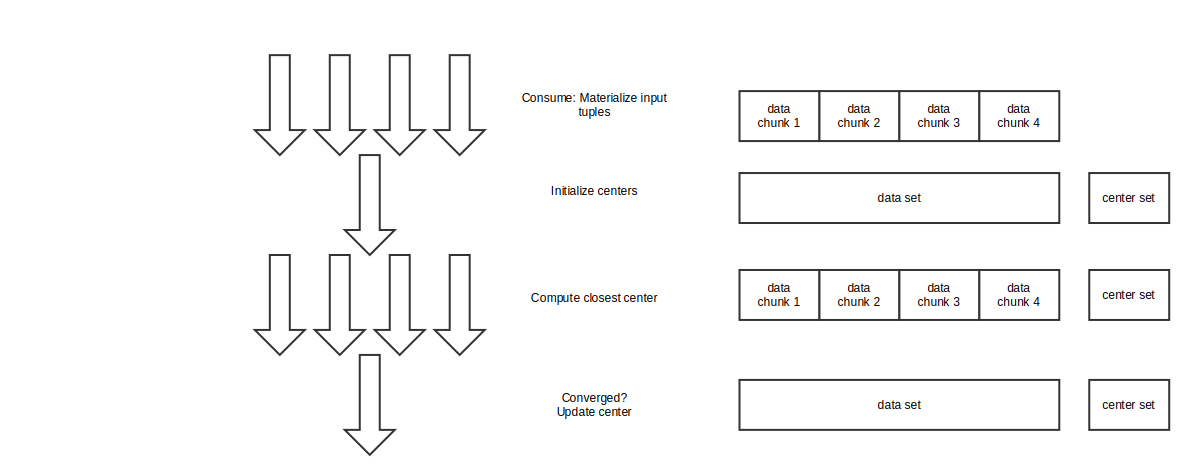
\includegraphics[scale=0.3]{figures/parallel}
  \caption[par]{par}
  \label{fig:parallel}
\end{figure}

After consuming the data our k-Means algorithm continues with finding the initial center set. For that, we have to break with our parallelism. For random initialization of the clusters, we have to select from the entire data set. This is even more important  for k-Means++ initialization. While we could select random data points for the the center just from one data chunk, this is not possible for the k-Means++ initialization strategy. Therefore, we have to create a global vector storing pointers to all materialization tuples. Now we can select the global center points by one of our initialization strategies and continue the parallel program sequence.
After the initialization we can now compute the distance for each data point to each center point. This can now be done in parallel. For each data chunk, we compute the distance on a separate thread. Without any overhead for process creation and management, this could lead to a running time of  this step of one fourth of the serial execution.
Afterwards, we go back to a serial execution of the program and check for each thread if the program converged. Only if all threads converged, we can terminate the algorithm and output the result of the clustering. Otherwise, we update the global centers by the newly assigned data points. In the first version of this work, this step is done in serial, but here is also potential to parallelize the program.
In the experiment section we will evaluate the parallel k-Means with the serial implementations. Even though only one part of the algorithm is parallelized and with the overhead of introduced by the parallelism, we expect performance gains.





